\documentclass[11pt]{amsart}
\usepackage[letterpaper]{geometry}
\usepackage{graphicx}
\usepackage{amssymb}
\usepackage{amsmath}
\usepackage{epstopdf}
\usepackage{fullpage}
\DeclareGraphicsRule{.tif}{png}{.png}{`convert #1 `dirname #1`/`basename #1 .tif`.png}

\newcommand{\solution}{\par\noindent\textbf{Solution.}\ }
\newcommand{\graphplaceholder}[1]{%
\begin{center}
\fbox{\parbox[c][2.15in][c]{0.82\textwidth}{\centering\textbf{Graph Placeholder}\\[0.5em]#1}}
\end{center}}

%%% BEGIN DOCUMENT
\begin{document}
\begin{center}
\Large Math 252, Fourth Examination---\small Review with Solutions\normalsize\vspace{.1in}
\end{center}

\small
\textbf{Directions:} Respond to each question by showing all work and fully justifying your solution. Your justification should include any well-known theorems, formulas, or mathematical properties used. \textbf{You may use an entire page for each problem, including both the front and back.} Only a \textbf{TI-30XII} scientific calculator may be used; \textbf{Casio calculators are not permitted}. If you use a calculator for a calculation, you must also show the expression or calculation entered to obtain your result. Answers submitted without sufficient supporting work or justification may receive little or no credit.

\begin{enumerate}

\item Let the curve $C$ be given by $x=-3\sin 2t$ and $y=3\cos 2t$ for $0\leq t\leq 3\pi$.
\begin{enumerate}
\item By eliminating the parameter $t$, find the equation of the circle (centered at the origin) in rectangular coordinates.

\solution
Squaring the two parametric equations gives
\[
x^2=9\sin^2(2t)
\qquad\text{and}\qquad
y^2=9\cos^2(2t).
\]
Therefore,
\[
x^2+y^2=9\bigl(\sin^2(2t)+\cos^2(2t)\bigr)=9.
\]
Thus, the rectangular equation is
\[
\boxed{x^2+y^2=9}.
\]

\item Determine the direction in which the circle is traversed and the number of revolutions completed over the interval.

\solution
The equations may be rewritten as
\[
x=3\cos\left(\frac{\pi}{2}+2t\right),
\qquad
y=3\sin\left(\frac{\pi}{2}+2t\right).
\]
Hence the polar angle is
\[
\theta=\frac{\pi}{2}+2t,
\]
which increases as $t$ increases. Therefore, the circle is traversed \textbf{counterclockwise}.

As $t$ increases from $0$ to $3\pi$, the angle increases by
\[
\Delta\theta=2(3\pi)-2(0)=6\pi.
\]
Since one revolution corresponds to an angle of $2\pi$,
\[
\frac{6\pi}{2\pi}=3.
\]
Thus, the curve is traversed counterclockwise for
\[
\boxed{3\text{ complete revolutions}}.
\]
\end{enumerate}

\item Let the curve $C$ be given by $x=-2+3t$ and $y=2-3t$ for all $t$.
\begin{enumerate}
\item By eliminating the parameter $t$, determine an equation relating $x$ and $y$.

\solution
From $x=-2+3t$, we obtain
\[
3t=x+2.
\]
Substituting this into the equation for $y$ gives
\[
y=2-3t=2-(x+2)=-x.
\]
Therefore, an equation relating $x$ and $y$ is
\[
\boxed{y=-x},
\]
or equivalently, $\boxed{x+y=0}$.

\item Sketch a graph of $C$, indicating the direction.

\solution
Because
\[
\frac{dx}{dt}=3>0
\qquad\text{and}\qquad
\frac{dy}{dt}=-3<0,
\]
the $x$-coordinate increases and the $y$-coordinate decreases as $t$ increases. Thus, the line is traversed from the upper left toward the lower right.

\begin{center}
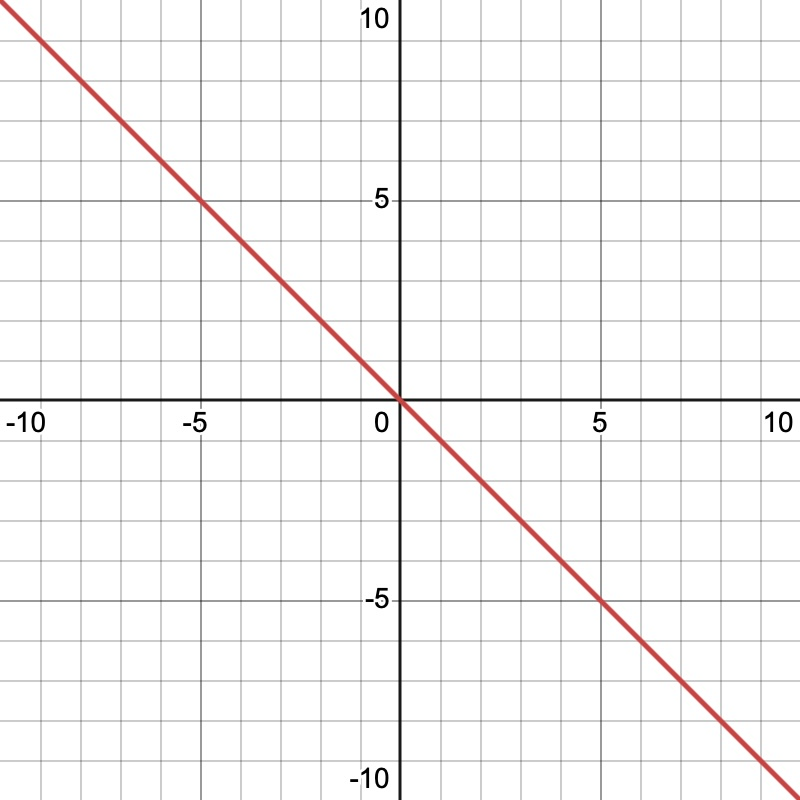
\includegraphics[scale=0.25]{Problem_2}
\end{center}
\end{enumerate}

\item Let the curve $C$ be defined parametrically by
\[
x=t^3-3t,
\qquad
y=t^2-2,
\qquad -2\leq t\leq 2.
\]
\begin{enumerate}
\item Find an expression for $\dfrac{dy}{dx}$ in terms of $t$.

\solution
Differentiate both coordinates with respect to $t$:
\[
\frac{dx}{dt}=3t^2-3=3(t^2-1)
\qquad\text{and}\qquad
\frac{dy}{dt}=2t.
\]
Therefore,
\[
\frac{dy}{dx}
=\frac{dy/dt}{dx/dt}
=\boxed{\frac{2t}{3(t^2-1)}},
\qquad t\neq \pm1.
\]

\item Determine all points $(x,y)$ on $C$ at which the tangent line is horizontal, and all points $(x,y)$ on $C$ at which the tangent line is vertical.

\solution
A horizontal tangent occurs when
\[
\frac{dy}{dt}=0
\qquad\text{and}\qquad
\frac{dx}{dt}\neq 0.
\]
Since $2t=0$, we have $t=0$. At $t=0$,
\[
\frac{dx}{dt}=-3\neq 0,
\]
and
\[
x=0^3-3(0)=0,
\qquad
y=0^2-2=-2.
\]
Thus, the curve has a horizontal tangent at
\[
\boxed{(0,-2)}.
\]

A vertical tangent occurs when
\[
\frac{dx}{dt}=0
\qquad\text{and}\qquad
\frac{dy}{dt}\neq 0.
\]
Solving $3(t^2-1)=0$ gives $t=\pm1$.

For $t=1$,
\[
x=1-3=-2,
\qquad y=1-2=-1.
\]
For $t=-1$,
\[
x=-1+3=2,
\qquad y=1-2=-1.
\]
In both cases, $dy/dt=2t\neq0$. Therefore, the vertical tangents occur at
\[
\boxed{(-2,-1)\text{ and }(2,-1)}.
\]
\end{enumerate}

\item Let the curve $C$ be defined parametrically by
\[
x=t^3,
\qquad y=t^4,
\qquad -2\leq t\leq 2.
\]
\begin{enumerate}
\item Determine whether the curve $C$ is smooth. Justify your answer.

\solution
The component functions have continuous derivatives on $[-2,2]$:
\[
\frac{dx}{dt}=3t^2
\qquad\text{and}\qquad
\frac{dy}{dt}=4t^3.
\]
At $t=0$,
\[
\frac{dx}{dt}=0
\qquad\text{and}\qquad
\frac{dy}{dt}=0.
\]
Because both derivatives are zero at the same parameter value, the curve is not smooth on the entire interval. Therefore,
\[
\boxed{C\text{ is not smooth on }[-2,2].}
\]
It is smooth on $[-2,0)$ and $(0,2]$.

\item Show that the point $(0,0)$ has both a horizontal tangent line and a vertical tangent line.

\solution
As written, this statement is not true for the given curve. For $t\neq0$,
\[
\frac{dy}{dx}
=\frac{4t^3}{3t^2}
=\frac{4t}{3}.
\]
Therefore,
\[
\lim_{t\to0}\frac{dy}{dx}=0,
\]
so the tangent line at $(0,0)$ is horizontal and has equation
\[
\boxed{y=0}.
\]
Eliminating the parameter gives
\[
y=t^4=(t^3)^{4/3}=x^{4/3},
\]
and the derivative of this rectangular equation also approaches $0$ at the origin. The curve does \emph{not} have a vertical tangent at $(0,0)$.

\medskip
\noindent\textbf{Instructor note:} The parametric equations must be changed if the intended conclusion is that the same point has both a horizontal and a vertical tangent.
\end{enumerate}

\item Let the curve $C$ be given parametrically by $x=1-t^2$ and $y=1+t^3$, for $0\leq t\leq 1$. Find the length $L$ of $C$.

\solution
The arc length of a parametric curve is
\[
L=\int_a^b\sqrt{\left(\frac{dx}{dt}\right)^2+
\left(\frac{dy}{dt}\right)^2}\,dt.
\]
Here,
\[
\frac{dx}{dt}=-2t
\qquad\text{and}\qquad
\frac{dy}{dt}=3t^2.
\]
Thus,
\begin{align*}
L
&=\int_0^1\sqrt{4t^2+9t^4}\,dt\\
&=\int_0^1 t\sqrt{4+9t^2}\,dt,
\end{align*}
where $t\geq0$ on the interval of integration.

Let
\[
u=4+9t^2,
\qquad du=18t\,dt.
\]
Then
\begin{align*}
L
&=\frac{1}{18}\int_4^{13}u^{1/2}\,du\\
&=\frac{1}{18}\left[\frac{2}{3}u^{3/2}\right]_4^{13}\\
&=\frac{1}{27}\left(13^{3/2}-4^{3/2}\right).
\end{align*}
Since $4^{3/2}=8$,
\[
\boxed{L=\frac{13\sqrt{13}-8}{27}}.
\]

\item Let the curve $C$ be given parametrically by $x=e^t\sin t$ and $y=e^t\cos t$, for $0\leq t\leq\pi$. Find the length $L$ of $C$.

\solution
Differentiate:
\[
\frac{dx}{dt}=e^t(\sin t+\cos t)
\]
and
\[
\frac{dy}{dt}=e^t(\cos t-\sin t).
\]
Therefore,
\begin{align*}
\left(\frac{dx}{dt}\right)^2+
\left(\frac{dy}{dt}\right)^2
&=e^{2t}\left[(\sin t+\cos t)^2+(\cos t-\sin t)^2\right]\\
&=e^{2t}(2\sin^2t+2\cos^2t)\\
&=2e^{2t}.
\end{align*}
Hence,
\begin{align*}
L
&=\int_0^\pi\sqrt{2e^{2t}}\,dt\\
&=\sqrt{2}\int_0^\pi e^t\,dt\\
&=\sqrt{2}\left[e^t\right]_0^\pi.
\end{align*}
Thus,
\[
\boxed{L=\sqrt{2}\left(e^\pi-1\right)}.
\]

\item Consider the rose $r=2\sin(3\theta)$.
\begin{enumerate}
\item Sketch a graph of the rose.

\solution
Because the coefficient of $\theta$ is $3$, the curve has three petals. One petal is traced for
\[
0\leq\theta\leq\frac{\pi}{3},
\]
and is centered at $\theta=\pi/6$. The remaining petals are obtained by rotations of $2\pi/3$.

\begin{center}
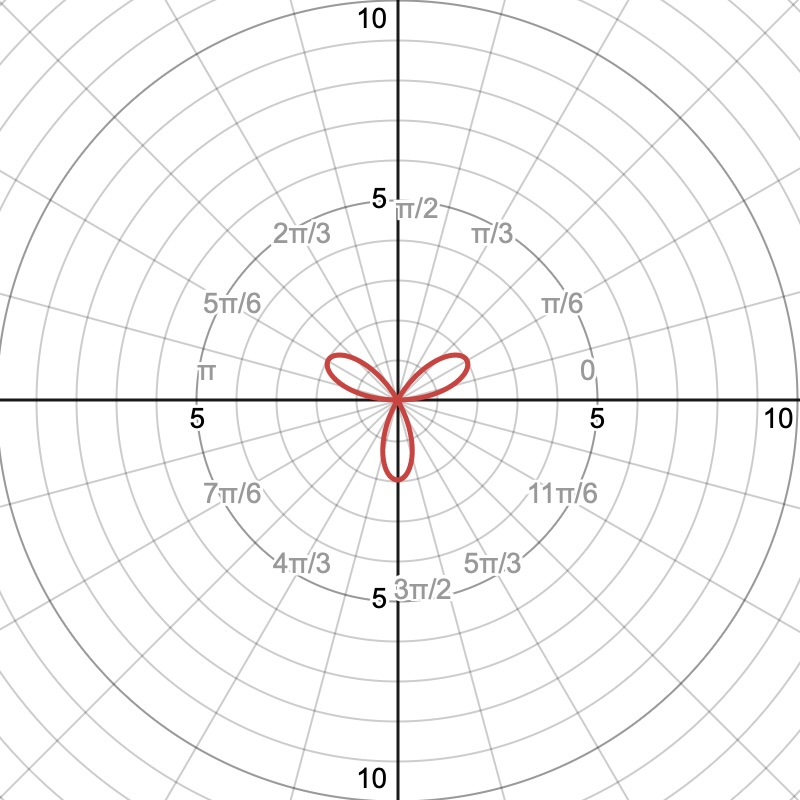
\includegraphics[scale=0.25]{Problem_7}
\end{center}
\item Write an integral and evaluate it for the area lying inside one petal of the rose. You may use $\displaystyle \sin^2x=\frac{1-\cos 2x}{2}$.

\solution
One petal is traced from $\theta=0$ to $\theta=\pi/3$. Using the polar-area formula,
\begin{align*}
A
&=\frac12\int_0^{\pi/3}r^2\,d\theta\\
&=\frac12\int_0^{\pi/3}\left(2\sin3\theta\right)^2\,d\theta\\
&=2\int_0^{\pi/3}\sin^2(3\theta)\,d\theta.
\end{align*}
Using the power-reduction identity,
\begin{align*}
A
&=\int_0^{\pi/3}\left(1-\cos6\theta\right)\,d\theta\\
&=\left[\theta-\frac16\sin6\theta\right]_0^{\pi/3}\\
&=\frac{\pi}{3}.
\end{align*}
Therefore,
\[
\boxed{A=\frac{\pi}{3}}.
\]
\end{enumerate}

\item Consider the cardioid $r=2+2\sin\theta$.
\begin{enumerate}
\item Sketch a graph of the cardioid.

\solution
The curve is symmetric about the vertical axis. It has a cusp at the origin when $\theta=3\pi/2$ and reaches its greatest radius, $r=4$, when $\theta=\pi/2$.

\begin{center}
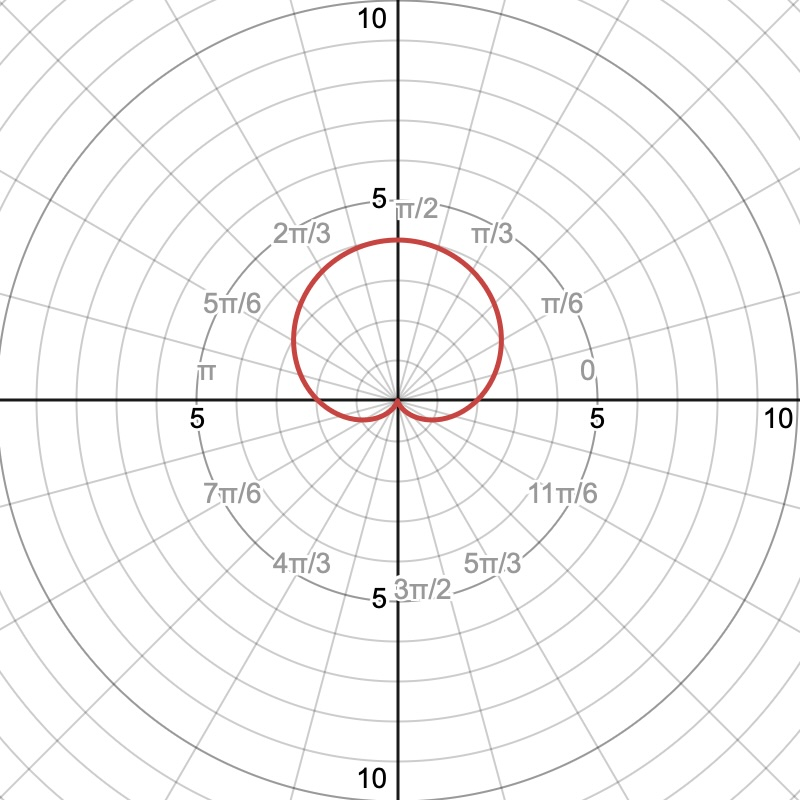
\includegraphics[scale=0.25]{Problem_8}
\end{center}
\item Write an integral and evaluate it for the area lying inside the cardioid.

\solution
The entire cardioid is traced once for $0\leq\theta\leq2\pi$. Therefore,
\begin{align*}
A
&=\frac12\int_0^{2\pi}(2+2\sin\theta)^2\,d\theta\\
&=2\int_0^{2\pi}\left(1+2\sin\theta+\sin^2\theta\right)\,d\theta.
\end{align*}
Over $[0,2\pi]$,
\[
\int_0^{2\pi}1\,d\theta=2\pi,
\qquad
\int_0^{2\pi}\sin\theta\,d\theta=0,
\qquad
\int_0^{2\pi}\sin^2\theta\,d\theta=\pi.
\]
Thus,
\[
A=2(2\pi+0+\pi)=\boxed{6\pi}.
\]
\end{enumerate}

\item Consider the lima\c{c}on $r=1+2\cos\theta$.
\begin{enumerate}
\item Sketch a graph of the lima\c{c}on.

\solution
The curve is symmetric about the polar axis. Since the coefficient of $\cos\theta$ is larger than the constant term, the curve has an inner loop. The curve passes through the pole when
\[
1+2\cos\theta=0,
\]
so
\[
\theta=\frac{2\pi}{3}
\qquad\text{or}\qquad
\theta=\frac{4\pi}{3}.
\]

\begin{center}
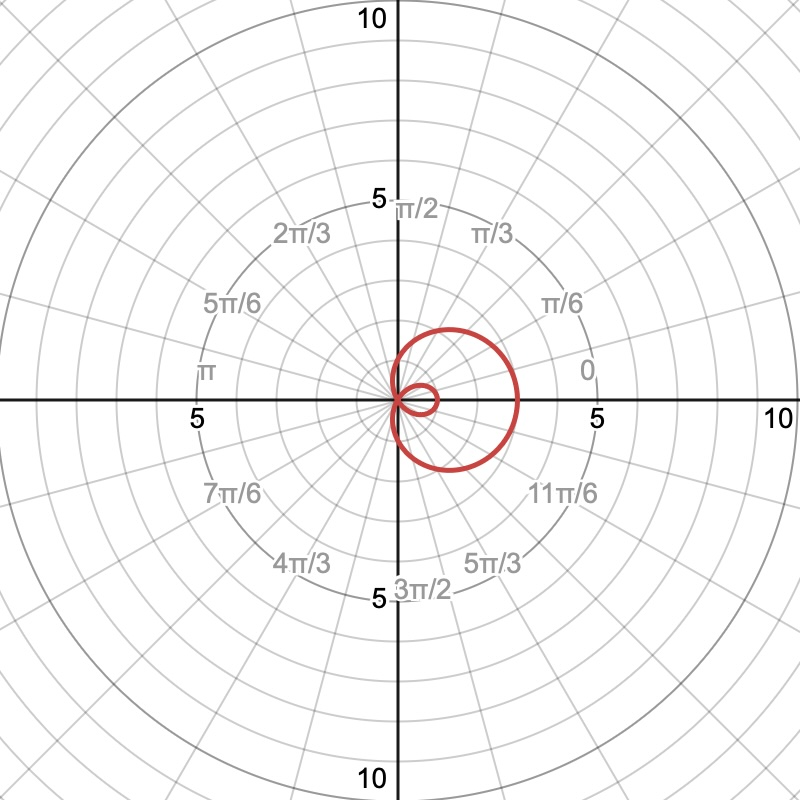
\includegraphics[scale=0.25]{Problem_9}
\end{center}

\item Write an integral and evaluate it for the area of the outer loop.

\solution
The outer loop is traced while $r\geq0$, which occurs for
\[
-\frac{2\pi}{3}\leq\theta\leq\frac{2\pi}{3}.
\]
Therefore,
\begin{align*}
A
&=\frac12\int_{-2\pi/3}^{2\pi/3}(1+2\cos\theta)^2\,d\theta\\
&=\frac12\int_{-2\pi/3}^{2\pi/3}
\left(1+4\cos\theta+4\cos^2\theta\right)\,d\theta\\
&=\frac12\int_{-2\pi/3}^{2\pi/3}
\left(3+4\cos\theta+2\cos2\theta\right)\,d\theta.
\end{align*}
Thus,
\begin{align*}
A
&=\frac12\left[3\theta+4\sin\theta+\sin2\theta\right]_{-2\pi/3}^{2\pi/3}\\
&=\frac12\left(4\pi+3\sqrt3\right).
\end{align*}
Therefore,
\[
\boxed{A=2\pi+\frac{3\sqrt3}{2}}.
\]
\end{enumerate}

\end{enumerate}

\end{document}
